\documentclass{article}
\usepackage{graphicx,tikz}
\usepackage{SIunits}
\usepackage[graphics,tightpage,active]{preview}
\PreviewEnvironment{tikzpicture}
\newlength\imagewidth
\newlength\imagescale
\begin{document}

\pgfmathsetlength{\imagewidth}{\linewidth} % desired displayed width of image
\pgfmathsetlength{\imagescale}{\imagewidth/670} % pixel width of image
\usetikzlibrary{shapes.arrows}
%
%% adjust scale of tikzpicture (and direction of y) such that pixel
%% coordinates can be used for drawing overlays:
\begin{tikzpicture}[x=\imagescale,y=-\imagescale]

% place image (integer coordinates refer to pixel centers):
\node[anchor=north west,inner sep=0pt,outer sep=0pt] at (0,0)
  {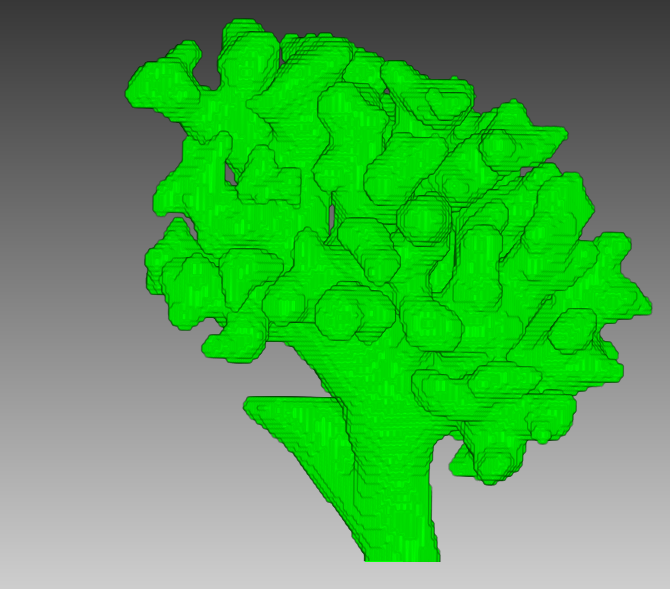
\includegraphics[width=\imagewidth]{segment-crop0041}};

%\draw (100,500) node ;
\draw[|-|,thick] (25,500) -- (175,500) node[midway,above] {\unit{300}{\micro\meter}};
\end{tikzpicture}

\end{document}